
\subsection{Layer Operating System}
Back-end will served on a Linux operating system on AWS Cloud platform.
\subsection{Layer Software Dependencies}
The back-end will be hosted using JavaScript's NodeJS Framework.
\begin{figure}[h!]
	\centering
 	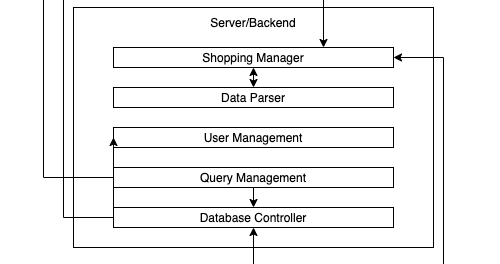
\includegraphics[width=0.60\textwidth]{images/backend}
 \caption{Back-End layer subsystem}
\end{figure}

\subsection{Shopping manager Subsystem}
The shopping manager subsystem will deal with all the shopping related computation. It will get requests
directly from the shopping subsystem of the front end. Then it will get the required shopping data
from the Data Controller layer, use the Data parser subsystem to parse the data into standard format,
and then send it as a response to the front-end.

\begin{figure}[h!]
	\centering
 	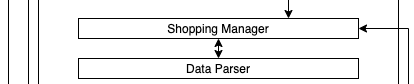
\includegraphics[width=0.60\textwidth]{images/ShoppingManager.png}
 \caption{Shopping manager Subsystem}
\end{figure}


\subsubsection{Subsystem Software Dependencies}
The subsystem will use the axios library to communicate with the Data Controller Layer.It will also use google maps library to display and calculate the optimum route to the user.

\subsubsection{Subsystem Programming Languages}
JavaScript (NodeJS)

\subsubsection{Subsystem Data Structures}
It will provide front end with the Prices and Availability of grocery items. Also the data required to display the optimum route on the front end.

\subsubsection{Subsystem Data Processing}
A description of any algorithms or processing strategies that are worth discussing for the subsystem. If you are implementing a well-known algorithm, list it. If it is something unique to this project, discuss it in greater detail. 
(Note: Ask Andrew about this)


\subsection{User Management Subsystem}
The user management subsystem will handle all requests from the front end related to the user of the
application and give back appropriate response. It will keep track of the currently logged in user.

\begin{figure}[h!]
	\centering
 	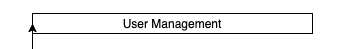
\includegraphics[width=0.60\textwidth]{images/UserManagement.png}
 \caption{User Management Subsystem}
\end{figure}


\subsubsection{Subsystem Software Dependencies}
This subsystem will Handle GoogleLogin authentication to make sure user is logged in and connect his google ID to the ID stored in the database. This subsystem will also use Axios library.

\subsubsection{Subsystem Programming Languages}
JavaScript (NodeJS) and some SQL

\subsubsection{Subsystem Data Structures}
This subsystem will create a data structure for the users profile using the google ID and send it to the front end.

\subsubsection{Subsystem Data Processing}
It will take in google ID for the user, search for that stored google ID in the database and pull all the data required data associated to that user.

\subsection{Query Management Subsystem}
The query management subsystem will handle all requests from the front end that needs a result from
a query on the database and give back the appropriate response.

\begin{figure}[h!]
	\centering
 	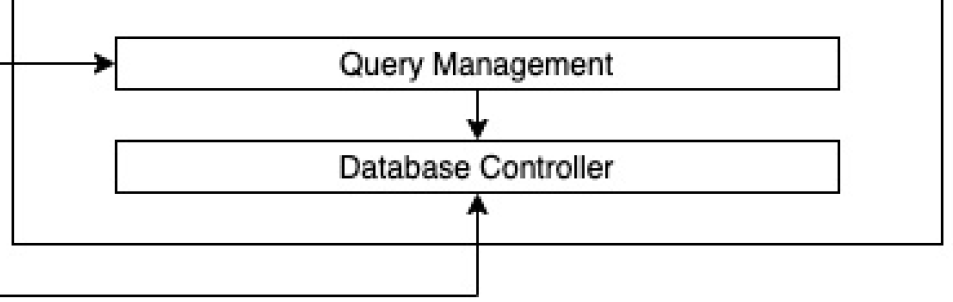
\includegraphics[width=0.60\textwidth]{images/Screenshot (61).png}
 \caption{Query Management Subsystem}
\end{figure}


\subsubsection{Subsystem Software Dependencies}
It will use the npm pg library to communicate with the postgreSQL Database stored in AWS RDS.

\subsubsection{Subsystem Programming Languages}
JavaScript (NodeJS) and queries written in SQL

\subsubsection{Subsystem Data Structures}
This subsystem will be responsible for creating and managing all the queries to the database.

\subsubsection{Subsystem Data Processing}
Depending on the request this layer will create a database query and send it to the database controller layer.

\subsection{Database Controller Subsystem}
The database controller will handle all the communication of the application to the database. It will
give responses to the query management system with the required data extracted from the database.

% \begin{figure}[h!]
% 	\centering
%  	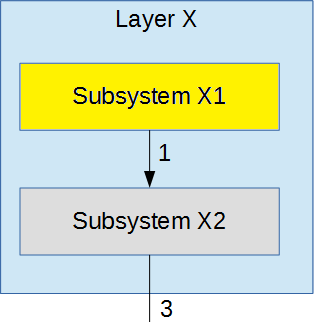
\includegraphics[width=0.60\textwidth]{images/subsystem}
%  \caption{Example subsystem description diagram}
% \end{figure}


\subsubsection{Subsystem Software Dependencies}
It will use the npm pg library to communicate with the postgreSQL Database stored in AWS RDS using axios.

\subsubsection{Subsystem Programming Languages}
JavaScript (NodeJS) and queries written in SQL

\subsubsection{Subsystem Data Structures}
This subsystem will take queries from the query management layer and send those queries to the database.

\subsubsection{Subsystem Data Processing}
This subsystem will send the queries to the database and get the result and send it back to the query management layer.